\chapter{基于OpenGL的深度相机仿真环境搭建}

\section{概述}
大数据驱动下的模型等训练需要大量带有人工标注真值的数据作为基础。深度相机作为近几年流行起来的新型相机,能够获取除了颜色意外的额外的视觉信息,极大促进了物体位姿估计领域的研究发展。物体位姿估计领域内越累越多的基于深度相机采集的深度图像的算法被提出并取得了不错的效果。但是这些物体位姿估计算法很难应用到实际生产生活中去,有一个很大的原因在于这些算法都依赖带有真值标注等训练数据,而这些带有真值的训练数据非常难以获取。有真值标注的训练数据的可获取性和易获取程度极大的影响到了物体位姿估计算法的进一步发展,因此本章将针对这一点,讨论一个基于OpenGL平台的深度相机仿真环境。

本章的主旨在于能够通过任意指定一个刚性物体的3D数据文件,便可以借助OpenGL计算模拟深度相机,自动并且快速地给出大量带有真值标注的深度相机仿真深度数据。由于本文研究内容主要在于位姿估计方面,因此本文给出的深度相机仿真环境给出的数据主要有仿真深度图像以及给定物体在仿真相机下的6维位姿$P$。其中这6维位姿包括以相机参考系为参考系下的物体的欧几里得坐标($P_x,P_y,P_z$),以及相机参考系下的欧拉角位姿($P_ax,P_ay,P_az$),如下图所示:

图图图图图图
\begin{figure}[htb]
	\centering 
	% 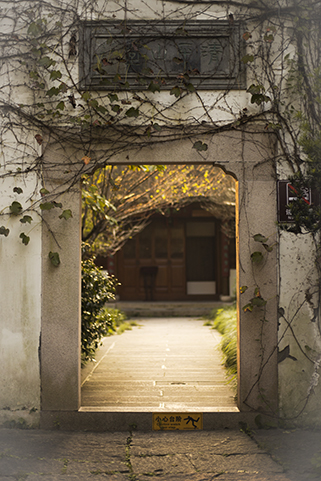
\includegraphics[width=\textwidth]{./Pictures/test.jpg} 
	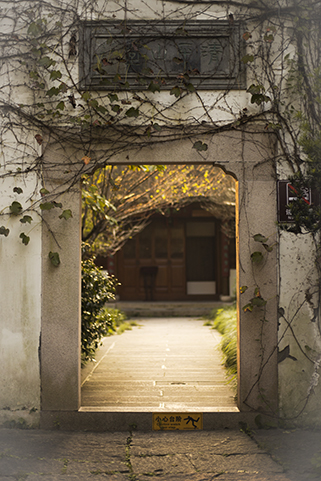
\includegraphics[scale=1.0]{./Pictures/test.jpg} 
	\caption{ljzst} 
\end{figure}

本章结构安排如下:3.2节主要介绍仿真环境中的数学模型,包括几何投影变换、坐标系的定义以及OpenGL平台中需要用到的一些基本理论。3.3节将阐述仿真环境搭建的具体流程以及如何改进仿真环境得到的数据,使仿真数据更加接近真实情况。最后在3.4节中通过具体的实验结果来验证得到的仿真数据的可行性。


\section{仿真数学模型}
% \subsection{两种几何变换}
在图像处理计算过程中,经常会遇到两种经典的变换,一种是仿射变换(Affine Transform),另一种是透视变换(Perspective Transform)。其中仿射变换是一种平面坐标系的伸缩旋转变换,是一种线形的变换,会保持原有图像的平行性,也就是说在原本图像中如果保持平行的两条直线,在经过仿射变换之后仍旧会保持平行。如下图:

图图图图图图
\begin{figure}[htb]
	\centering 
	% 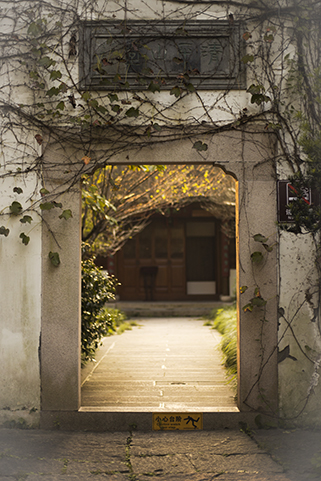
\includegraphics[width=\textwidth]{./Pictures/test.jpg} 
	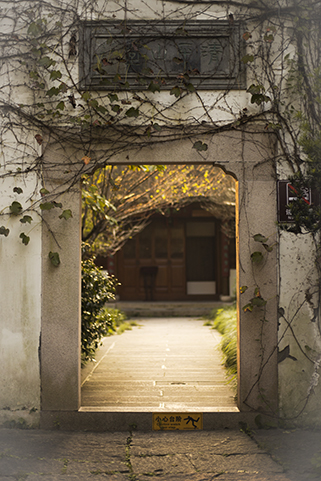
\includegraphics[scale=1.0]{./Pictures/test.jpg} 
	\caption{ljzst} 
\end{figure}

仿射变换的变换可以由一个$2*3$的矩阵$Rt_{affine}$来表达:
\begin{equation}
	Rt_{affine}=\left[R\quad T\right]=
	\left[
	\begin{aligned}
	r_{11}\quad r_{12}\quad t_1 \\
	r_{21}\quad r_{22}\quad t_2
	\end{aligned}
	\right]
\end{equation}
上式中$R$表示坐标系的旋转,$T$表示坐标系的平移。在仿射变换下,若给定一个点$P:(x,y)$,其仿射变换后将得到点$P':(x',y')$如下:
\begin{equation}
	[x'\quad y']^\top=Rt_{affine}\cdot [x\quad y\quad 1]^\top=
	\left[
	\begin{aligned}
	r_{11}\quad r_{12}\quad t_1 \\
	r_{21}\quad r_{22}\quad t_2
	\end{aligned}
	\right]\cdot 
	\left[
	\begin{aligned}
	x \\
	y \\
	1
	\end{aligned}
	\right]
\end{equation}
		
透视变换则是指利用透视中心、像点、目标点三点共线的条件,按透视旋转定律使承影面(透视面)绕迹线(透视轴)旋转某一角度,破坏原有的投影光线束,仍能保持承影面上投影几何图形不变的变换。透视变换本质上是一种三维空间上的投影变换,如下图所示:
\begin{figure}[htb]
	\centering 
	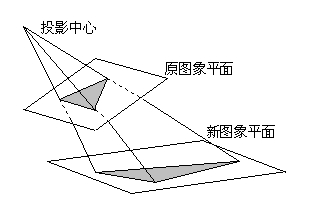
\includegraphics[scale=1.0]{./mypic/透视变换.jpg} 
	\caption{透视变换} 
\end{figure}

也就是说透视变换是将原始图像从三维空间投影到二维空间。例如给定一个初始点$P:(x,y,z)$,这个点投影到二维平面可以通过一个$3*3$的矩阵$P$表达:
\begin{equation}
	P=
	\left[
	\begin{aligned}
	a_{11}\quad a_{12}\quad a_{13} \\
	a_{21}\quad a_{22}\quad a_{23} \\
	a_{31}\quad a_{32}\quad a_{33}
	\end{aligned}
	\right]
\end{equation}
假设投影平面的坐标基表示为$(u,v)$,则有:
\begin{equation}
	\left[
	\begin{aligned}
	x \\
	y \\
	z
	\end{aligned}
	\right]=
	\left[
	\begin{aligned}
	a_{11}\quad a_{12}\quad a_{13} \\
	a_{21}\quad a_{22}\quad a_{23} \\
	a_{31}\quad a_{32}\quad a_{33}
	\end{aligned}
	\right]\cdot
	\left[
	\begin{aligned}
	u \\
	v \\
	1
	\end{aligned}
	\right]
\end{equation}
从而可以得到投影后的新坐标表达为:
\begin{equation}
\begin{aligned}
	x'=\frac{x}{z}=\frac{a_{11}u+a_{12}v+a_{13}}{a_{31}u+a_{32}v+a_{33}}
		=\frac{k_{11}u+k_{12}v+k_{13}}{k_{31}u+k_{32}v+1} \\
	y'=\frac{y}{z}=\frac{a_{21}u+a_{22}v+a_{23}}{a_{31}u+a_{32}v+a_{33}}
		=\frac{k_{21}u+k_{22}v+k_{23}}{k_{31}u+k_{32}v+1}
\end{aligned}
\end{equation}

对比上面两种变换方式可以看出,一个仿射变换最多需要有6个参数来确定,而一个投影变换的最多参数量达到了8个。投影变换相比仿射变换具有更高的复杂度,因此从模型简易角度来讲,利用仿射变换进行深度相机的仿真环境搭建更为简洁方便。一些点线扫描式的深度采集设备也是符合仿射变换模型进行深度图像采集的。

然而现实生活中,更多数量的深度相机原理大致可以分为两类,一种是基于结构光的,另一种是基于ToF(Time of Flight)的。基于结构光的深度相机通过发射结构光,并利用另一个相机采集到的视差信息构建深度图像。基于ToF的深度相机则是通过一个红外线激光发射器发射出红外线,再通过另一个红外线接收装置采集红外线照射到物体之后返回的时间,通过这个时间差来计算物体到达相机的距离。在这两种深度相机模型下,深度相机都可以被近似看作一个质点,也就是这些真实的深度相机都是以相机作为投影点,将物体深度信息投影到像平面上的到的深度图像。这一模型符合投影变换的框架,因此本文的仿真深度环境搭建也是基于投影变换进行搭建的。

下图为本文的仿真环境的一个简单几何说明图:
\begin{figure}[htb]
	\centering 
	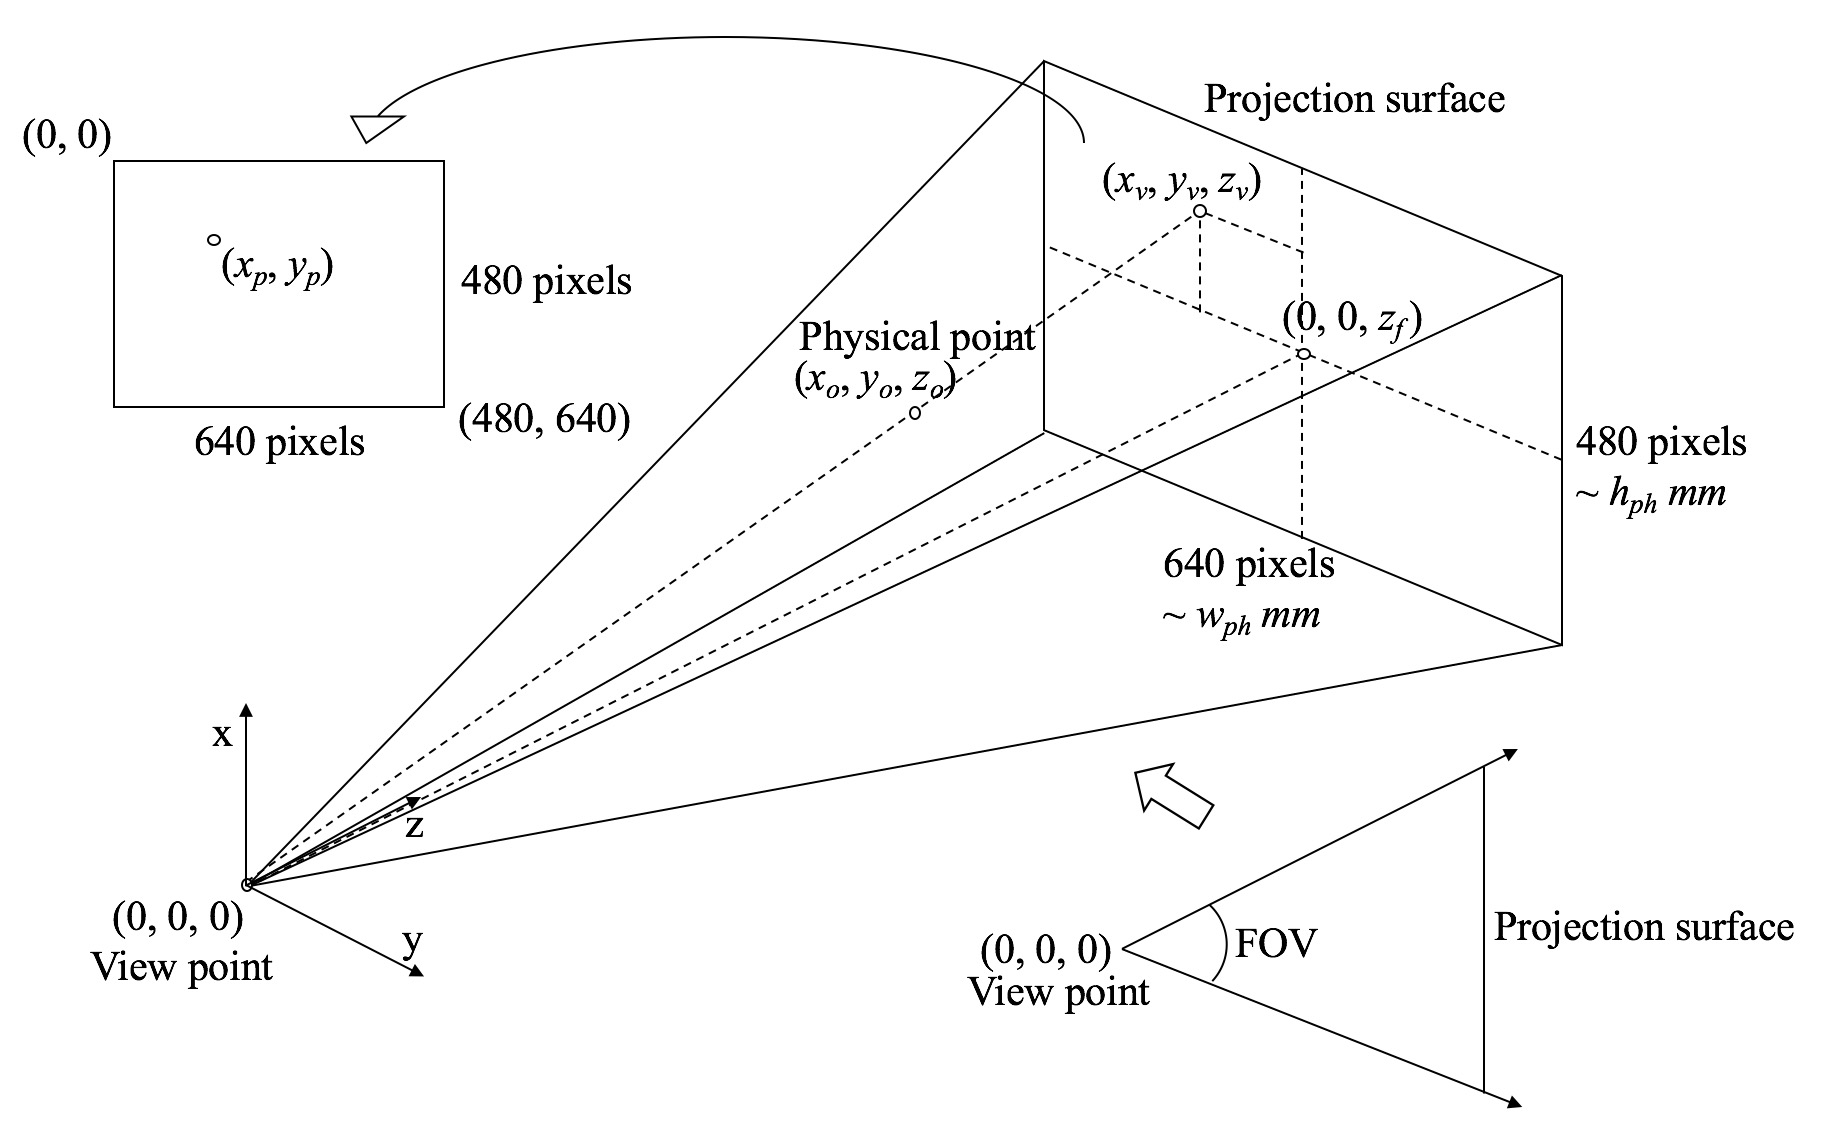
\includegraphics[width=\textwidth]{./mypic/projection.jpg} 
	\caption{仿真环境几何示例} 
\end{figure}

其中定义仿真相机位于世界坐标的原点$O$,也就是相机坐标系和世界坐标系重合。定义深度投影平面(Projection Surface)的分辨率为640*480像素。其中存在一个模拟物理点(Physical Point),记为$P_0:(x_0,y_0,z_0)$,其按照投影变换的规则将投影在投影平面上的点$P_v:(x_v,y_v,z_v)$处,并且原点$O$、模拟物理点$P_0$以及投影点$P_v$三点共线。因此存在如下等式:
\begin{equation}
	\frac{x_0}{x_v}=\frac{y_0}{y_v}=\frac{z_0}{z_v}
\end{equation}
图中涉及另外几个OpenGL的基本定义。投影平面(Projection Surface)具有事先给定的深度值$z_f$,并且垂直于相机坐标系下的$z$轴方向。像平面定义为标准VGA图像大小,也就是$640*480$分辨率大小,并且定义其横向从左往右为$x$轴方向,纵向从上往下为$y$方向。FOV(Field of View),也就是视场角。FOV定义为投影平面的上边界与下边界分别与相机坐标原点形成的角度,可以描述深度相机的视野角度。

有了上述基本定义之后,就可有如下几个等式:
\begin{equation}
\begin{aligned}
	\frac{pixels\ in\ width}{pixels\ in\ height}=
	\frac{640}{480}=
	\frac{w_{ph}}{h_{ph}} \\
	h_{ph}=2\cdot z_f \cdot \tan(FOV/2)
\end{aligned}
\end{equation}
其中$w_{ph}$和$h_{ph}$分别表示物理投影面的实际物理宽度和长度,从而对于模拟物理点$P_0:(x_0,y_0,z_0)$在深度图像中对应的像素位置关系为:
\begin{equation}
\begin{aligned}
	\frac{x_v}{h_{ph}/2}=\frac{pixels\ in\ height/2-x_p}{pixels\ in\ height/2} \\
	\frac{y_v}{w_{ph}/2}=\frac{pixels\ in\ width/2+y_p}{pixels\ in\ width/2}
\end{aligned}
\end{equation}
联立上述几个式子可以解得:
\begin{equation}
\begin{aligned}
	x_p=\left(1-\frac{x_0}{z_0\cdot\tan(FOV/2)}\right)\cdot \frac{pixels\ in\ height}{2} \\
	y_p=\left(\frac{y_0}{z_0\cdot\tan(FOV/2)}-1\right)\cdot \frac{pixels\ in\ width}{2}
\end{aligned}
\end{equation}

从上式可以看出,只要指定好FOV角度大小以及确定深度图像的分辨率大小,任意空间坐标$P_0:(x_0,y_0,z_0)$都可以直接计算的到投影变换下的像平面像素位置。

% \subsection{坐标系以及坐标系转换} % 四元数、参考系的转换等
% 深度相机仿真环境中,除了世界坐标系以外,每一个物体都有其本身的坐标系。在OpenGL环境中,我们将假想的深度相机置于世界坐标原点,并将深度相机坐标系与世界坐标系完全重合,从而可以有如下图所示的一个基本几何定义:
% \begin{figure}[htb]
% 	\centering 
% 	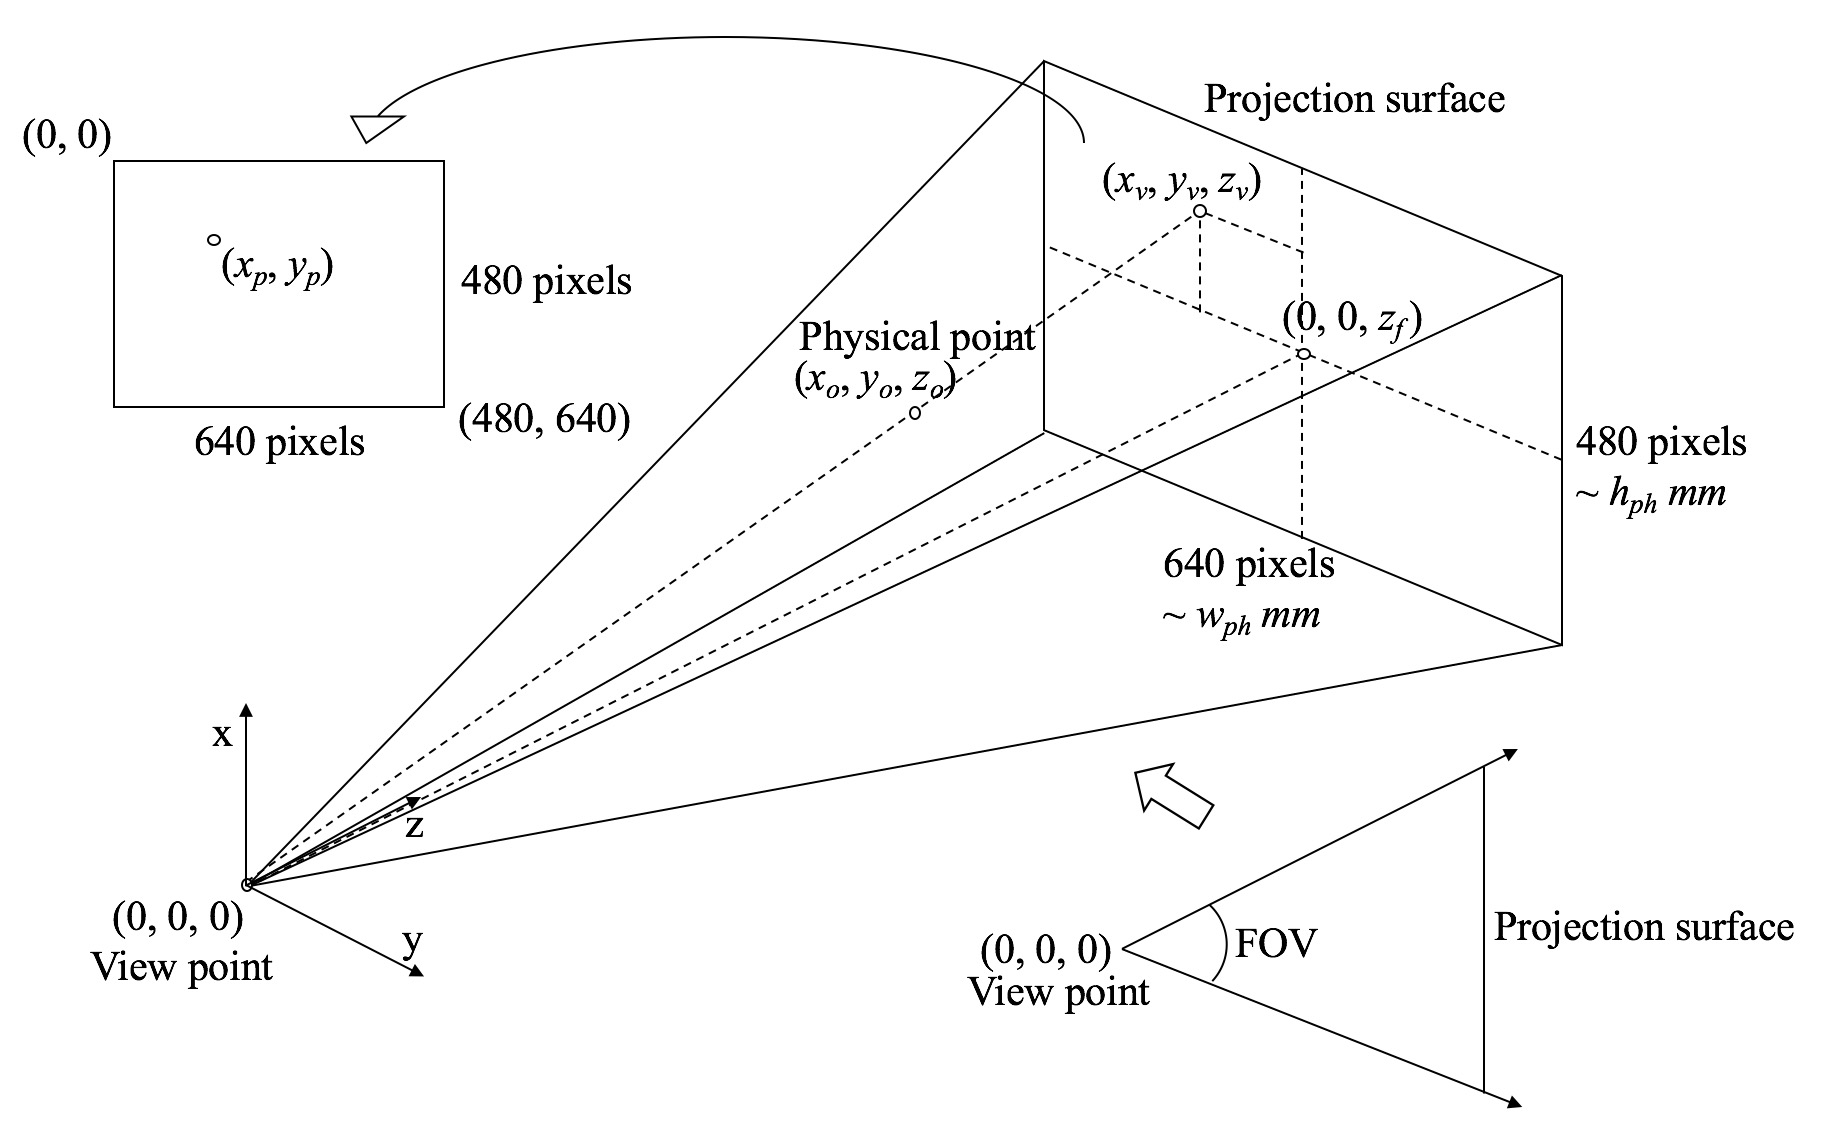
\includegraphics[width=\textwidth]{./mypic/projection.jpg} 
% 	\caption{} 
% \end{figure}
% \subsection{OpenGL原理} % stl文件、深度检测等等



\section{仿真环境搭建}
在有了上述投影变换的基本数学模型后,本节将继续阐述如何搭建一个实际的物理仿真平台。
\subsection{仿真流程及细节} % 
物体的3D模型文件是仿真环境中最重要的一个元素。3D文件可以有很多格式,例如3MF、STL、OBJ以及PLY等等文件格式,每种格式的文件都有其自身的特点,其中STL文件格式是一种非常通用简介的3D文件格式,并且与OpenGL平台相容性较好,因此本文就以STL文件为例进行阐述。

STL文件是由若干个三角形的相互连接定义组成,每个三角形平面的定义包括三角形各个顶点的三维坐标以及三角形平面的法向量,也就是这个三角形平面的朝向。其中这些顶点的三维坐标以及向量表达都是以该物体本身坐标系作为基准进行描述的,因此当我们需要仿真一个在空间中任意位置任意方向的物体的时候,需要将该物体的所有三角形坐标以及法向量进行变换。也就是存在一个物体坐标系到世界坐标系的变换:
\begin{equation}
	Cord_{obj}\to Cord_{world}
\end{equation}
描述这样一个变换通畅可以用六个维度进行定量衡量:X、Y、Z三个方向上的平移以及遵循一定顺序的X、Y、Z三方向的欧拉角旋转量。需要注意的是,仅仅给定了这六个变换参数也还是不能完全定义一个变换,还需要指定这些变换参数是在哪个参考系下进行的。本实验中采用的变换规则为:
\begin{enumerate}
\item 物体先以世界坐标系为基准进行X、Y、Z三个方向上的平移$\to State_1$
\item 物体以自身坐标系为基准,绕Z轴方向进行旋转$\to State_2$
\item 物体以自身坐标系为基准,绕X轴方向进行旋转$\to State_3$
\item 物体以自身坐标系为基准,绕Y轴方向进行旋转$\to State_4$
\end{enumerate}
例如给定了这六个参数分别为${d_x,d_y,d_z,a_x,a_y,a_z}$,并且初始情况下物体自身坐标系和世界坐标系重合,则物体坐标系下的一个点$P:{x,y,z}$经过变换后得到的世界坐标系下坐标可以有如下计算过程的到:

首先须要以自身坐标系为基准进行旋转,根据ZXY的顺序可以有旋转矩阵:
\begin{equation}
	R_{ZXY}=
	\begin{bmatrix} 
	cy\cdot cz-sy\cdot sx\cdot sz & cy\cdot sz+sy\cdot sx\cdot cz & -sy\cdot cx \\
	-sz\cdot cx & cz\cdot cx & sx \\
	sy\cdot cz+cy\cdot sx\cdot sz & sy\cdot sz-cy\cdot sx\cdot cz & cy\cdot cx 
	\end{bmatrix} 
\end{equation}
其中,$sx,cx,sy,cy,sz,cz$分别表示$sin(a_x),cos(a_x),sin(a_y),cos(a_y),sin(a_z),cos(a_z)$,旋转之后再进行平移便可得到最后世界坐标系下物体变换后的新坐标:
\begin{equation}
	P':\left[\begin{aligned}x' \\y' \\ z'\end{aligned}\right]=
	R_{ZXY}\cdot \left[\begin{aligned}x \\y \\ z\end{aligned}\right]+
	\left[\begin{aligned}dx \\dy \\ dz\end{aligned}\right]
\end{equation}
不同的变换顺序以及不同的基准坐标系都可以实现不同的变换,但在经过大量的实验测试之后可以发现,上述变换方式以及顺序与OpenGL默认环境最相容,在仿真过程中具有较强的直观感受,同时在计算上也具有较为简洁的中间步骤。

得益于OpenGL的Zbuffer机制,在对一个物体进行上述旋转变换后便可以很容易得到对应物体位姿下的深度仿真图以及对应的物体位姿真值。由于在OpenGL环境中,所有的深度数据都是通过Zbuffer来进行存储的,而Zbuffer的存储值取值范围受限于计算机仿真空间大小而被限制为$[0,1]$,其中0对应仿真环境中所能接受的最近点距离$near_z$,1对应仿真环境中所能接受的最远点距离$far_z$。因此这里存在一个转换关系:
\begin{equation}
	z=\frac{far_z\cdot near_z}{far_z - (far_z-near_z)\cdot z'}
\end{equation}
其中$z'$表示Zbuffer值$\to [0,1]$,$z$为真实物理长度距离。经过上式转换,就可以利用OpenGL环境得到最后真正的仿真深度图像。

下面为利用OpenGL进行深度图像仿真的基本流程图:
图图图图图图
\begin{figure}[htb]
	\centering 
	% 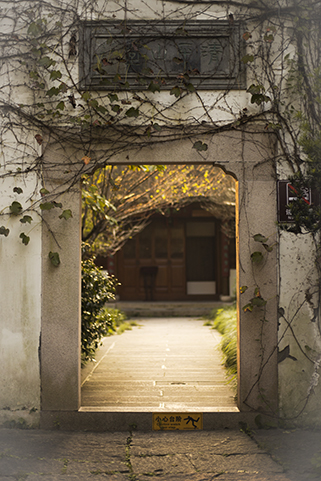
\includegraphics[width=\textwidth]{./Pictures/test.jpg} 
	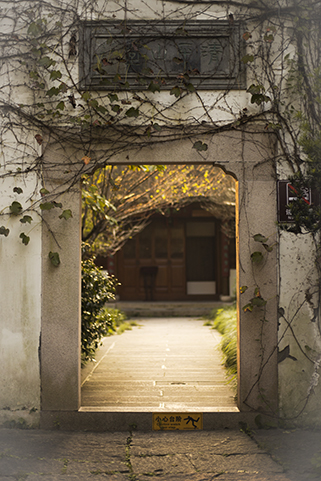
\includegraphics[scale=1.0]{./Pictures/test.jpg} 
	\caption{ljzst} 
\end{figure}





\subsection{模拟深度数据噪声} % 双高斯
可以发现,在上一小节中直接利用OpenGL可以得到非常完美的深度仿真图,该深度图像具有非常好的细节质量,没有任何噪声。但是对比下图可以发现,直接得到的深度图仿真图具有如下几个非常明显的缺点:

图图图图图图
\begin{figure}[htb]
	\centering 
	% 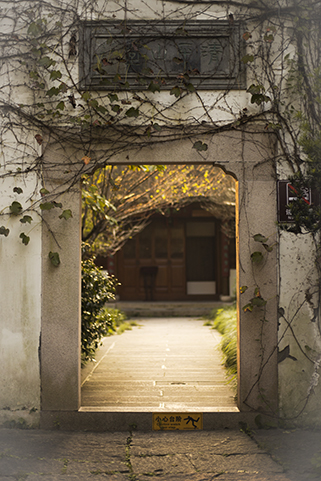
\includegraphics[width=\textwidth]{./Pictures/test.jpg} 
	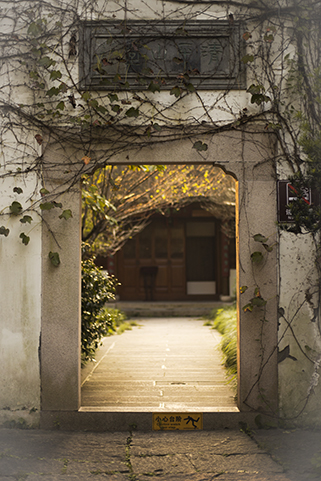
\includegraphics[scale=1.0]{./Pictures/test.jpg} 
	\caption{ljzst} 
\end{figure}
\begin{itemize}
\item 仿真深度图像非常光滑,没有任何噪声,但是真实深度图像有大量的噪声,即使是一个平面也会存在不平整的地方。
\item 仿真深度图像数据非常完备,所有像素点都存在数据,但是真实深度图像则有很多位置存在数据丢失,也就是真实深度图像存在数据空洞。
\item 仿真深度图像由于只仿真了物体本身的深度数据,除了物体本身的深度数据意外,其它位置的深度数据都是仿真环境的最远距离,没有实际意义。但是真实深度图像则有背景数据,甚至在一些情况下会有别的干扰物体对目标物体进行干扰或者遮挡。
\end{itemize}
上述问题的存在,使得仿真深度图由于太过完美而损失了大量真实性,对后续的仿真数据分析带来了极大的影响。因此本文针对这几点,提出了几个步骤对这些缺点进行修补,从而提高仿真图像的真实感,提升仿真真实性。

首先针对原始仿真图像没有任何噪声,极度光滑的问题,通畅可以采用模拟随机高斯噪声来解决。简单的高斯噪声可以通过对每一个像素点具有的深度值$d$附加一个均值为$0$,方差为$\sigma ^2$的高斯噪声得到。考虑到目前绝大多数的深度相机在测量上都存在一个和实际深度成正比的误差曲线,也就是随着被测物体的深度值越大,深度相机测量得到的深度信息携带的距离误差也会越大,因此此处$\sigma$应为一个与被测物体深度$\bar{d}$相关的函数,在本实验中采用下式表达形式:
\begin{equation}
	\sigma = \sqrt{\lambda \cdot \bar{d}}
\end{equation}
于是有:
\begin{equation}
	d'=d+N(0, \lambda \cdot \bar{d})
\end{equation}
但是,经过实验发现,仅仅采用简单的高斯噪声进行模拟得到的结果非常不理想。这样得到的仿真数据有非常明显的毛刺,在本该是平面的地方变得非常不光滑,或者说表面的法向量将存在非常严重的不连续性跳变。而实际深度图像中虽然存在噪声起伏,但是总体上还是平滑的,或者说表面法向量是基本不存在较大跳变的,如下图所示:

图图图图图图
\begin{figure}[htb]
	\centering 
	% 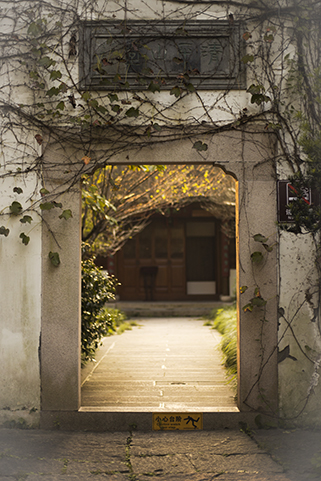
\includegraphics[width=\textwidth]{./Pictures/test.jpg} 
	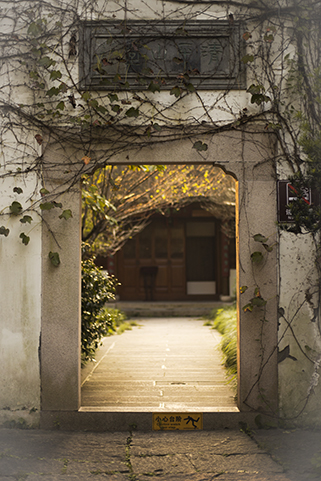
\includegraphics[scale=1.0]{./Pictures/test.jpg} 
	\caption{ljzst} 
\end{figure}

经过实验,本文最后采取适当调高$\lambda$的值,并在高斯噪声基础上套一层高斯平滑滤波。高斯平滑滤波可以采用一个比较大的高斯核进行操作,这样得到的复合高斯噪声就能有一个非常好的表现,既能够起到添加噪声的作用,同时也可以保证噪声的增加不会导致一些几何表面的眼中变形。最后可以用如下式子表示添加到原始仿真深度数据上的噪声:
\begin{equation}
	d'=d+Gaussian_{\Delta}(N(0, \lambda \cdot \bar{d}))
\end{equation}
其中$Gaussian_{\Delta}(\cdot)$表示对某一个$\Delta$区域上的高斯滤波操作。

针对第二点仿真深度图像没有空洞,但是实际深度图像存在较多空洞的问题。本文没有用直接的方法来生成空洞进行模拟,原因在于实际深度图像中很多的空洞的产生原因非常复杂,有外界环境红外光的干扰,也有物体表面材质的原因导致,如果直接通过随机的方式给仿真图像增加空洞,不光空洞大小会显得很突兀,空洞的形状也非常不好选择。因此,为了解决这个问题,本文采用逆向思维,通过修补真实深度图像数据中的空洞来使得其和仿真深度数据更加接近。

在大量的观察和对比,可以发现实际深度图像中绝大多数的空洞应有的深度值其实是和其周围数据接近或者完全一致的。也就是说这些空洞往往出现在物体的边界或者物体与物体之间的连接处,因此可以通过一些基本的图形学操作达到修补空洞的目的。基本的图形学操作有腐蚀、膨胀、开闭运算等。下图展示了一个具有空洞的图形经过简单的膨胀图像操作,将空洞填满。

图图图图图图
\begin{figure}[htb]
	\centering 
	% 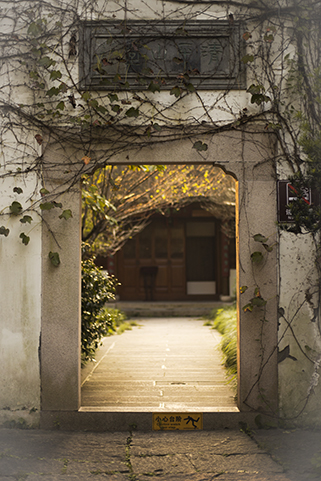
\includegraphics[width=\textwidth]{./Pictures/test.jpg} 
	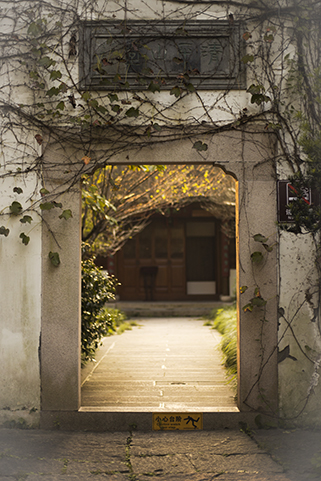
\includegraphics[scale=1.0]{./Pictures/test.jpg} 
	\caption{ljzst} 
\end{figure}

针对最后一点,实际深度图像具有背景以及前景遮挡等复杂环境而仿真环境得到的深度图像过于完美的情况。本文通过事先采集大量的背景深度数据(真实深度相机数据),随后将其叠加进原始仿真深度图像中去来解决复杂背景的模拟问题。用同样方法事先采集一些前景遮挡数据,并根据当前物体的仿真位置,将这些前景遮挡数据添加到其中进行模拟。其中,假设事先采集好的背景数据集合为$D_{bg}:\{d_{bg}^1,d_{bg}^2,...d_{bg}^n\}$,原始深度图像(经过噪声处理后的仿真深度图像)为$D_0$,则加入背景信息后的仿真深度图像可以表达为:
\begin{equation}
	D_1=union\{\ \max_{depth}\ (d_{bg}^i, D_0)\}
\end{equation}
进一步给定事先采集的前景数据集合为$D_{fg}:\{d_{fg}^1,d_{fg}^2,...d_{fg}^n\}$,物体在仿真环境中的位置为$P_{obj}$,则有加入前景遮挡信息后的仿真深度图像表示为:
\begin{equation}
\begin{aligned}
	\overline{d_{fg}^i} = F(P_{obj},d_{fg}^i)
	D_{final}=union\{\ \max_{depth}\ (\overline{d_{fg}^i}, D_1)\}
\end{aligned}
\end{equation}
其中$F(\cdot)$表示根据当前仿真物体的位姿调整前景物体信息到适当位置的变换函数,这个变换函数可以根据实际情况任意设置,因此不在此继续阐述。通过这种方式,在$F(\cdot)$尽量合理的情况下,就可以生成最后具有非常高仿真度的深度图像$D_{final}$。

下图整理为整个深度图像仿真流程概况图:

图图图图图图
\begin{figure}[htb]
	\centering 
	% 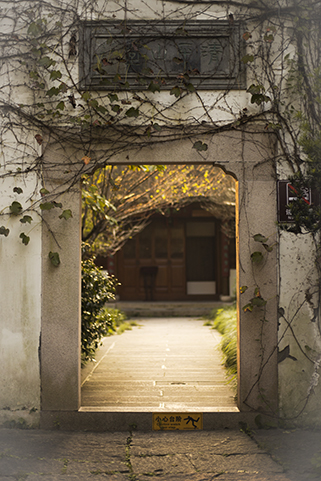
\includegraphics[width=\textwidth]{./Pictures/test.jpg} 
	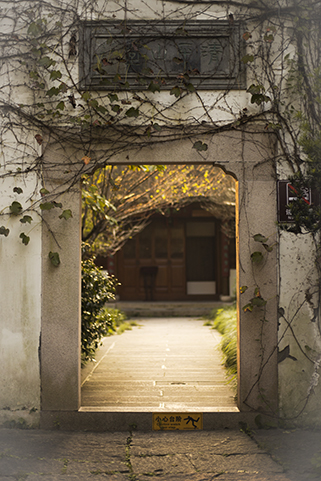
\includegraphics[scale=1.0]{./Pictures/test.jpg} 
	\caption{ljzst} 
\end{figure}






\section{实验结果与分析}











